%-------------------------------------------------------------------------------
% DRIVEN CAVITY FLOWS 
%-------------------------------------------------------------------------------

\section{2D driven Cavity Flows} \label{sec:driven_cav}

In two-dimensional (2D) driven cavity flows, a viscous Newtonian incompressible
fluid is confined within a square (or rectangular) domain. In these model
problems, the fluid is driven through the motion of the bounding walls. These
types of flow configurations have been widely used due to their simplicity and
relevance as benchmarks problem for validating numerical solvers and
investigating various flow phenomena.

A recent and comprehensive review conducted by \citet{kuhlmann2019} provides
insights for the extensive research carried out on the many variants of the
lid-driven cavity.

\subsection{The single lid-driven Cavity Flow}

The most basic configuration of the flow problem involves a square cavity where
only one wall, referred to as the lid, is in motion while the other walls
remain stationary. This simple 2D case has been extensively studied numerically
and serves as one of the canonical benchmark problems nowadays. The first
thorough computational investigation lies more than half a century back
\citep{burggraf1966}. Figure \ref{fig:cav_simple} shows the basic setup, and
figure \ref{fig:Re_cav_simple} illustrates the typical flow pattern for two
different Reynolds numbers. The depicted streamlines show a central vortex
driven by the upper lid's motion to the right. Therefore, the primary vortex
rotates clockwise. Moreover, the flow shows secondary vortices at the upper and
lower corners at higher Reynolds numbers ($8000$).

\begin{figure}[ht]
\centering
\begin{tikzpicture}[scale=1.5]
  \draw[thick] (0, 0) rectangle (2, 2);
  \draw[thick, pattern=north west lines, pattern color=gray] (0, 2)
    rectangle (2, 2.15);
  \draw[->, thick] (0.5, 2.25) -- (1.5, 2.25);
  
  \node at (1, 1) {Fluid};
  \node at (1, 2.3) [above] {Moving lid};
\end{tikzpicture}
\caption{Single lid-driven cavity}
\label{fig:cav_simple}
\end{figure}

\begin{figure}[ht!]
\begin{center}
  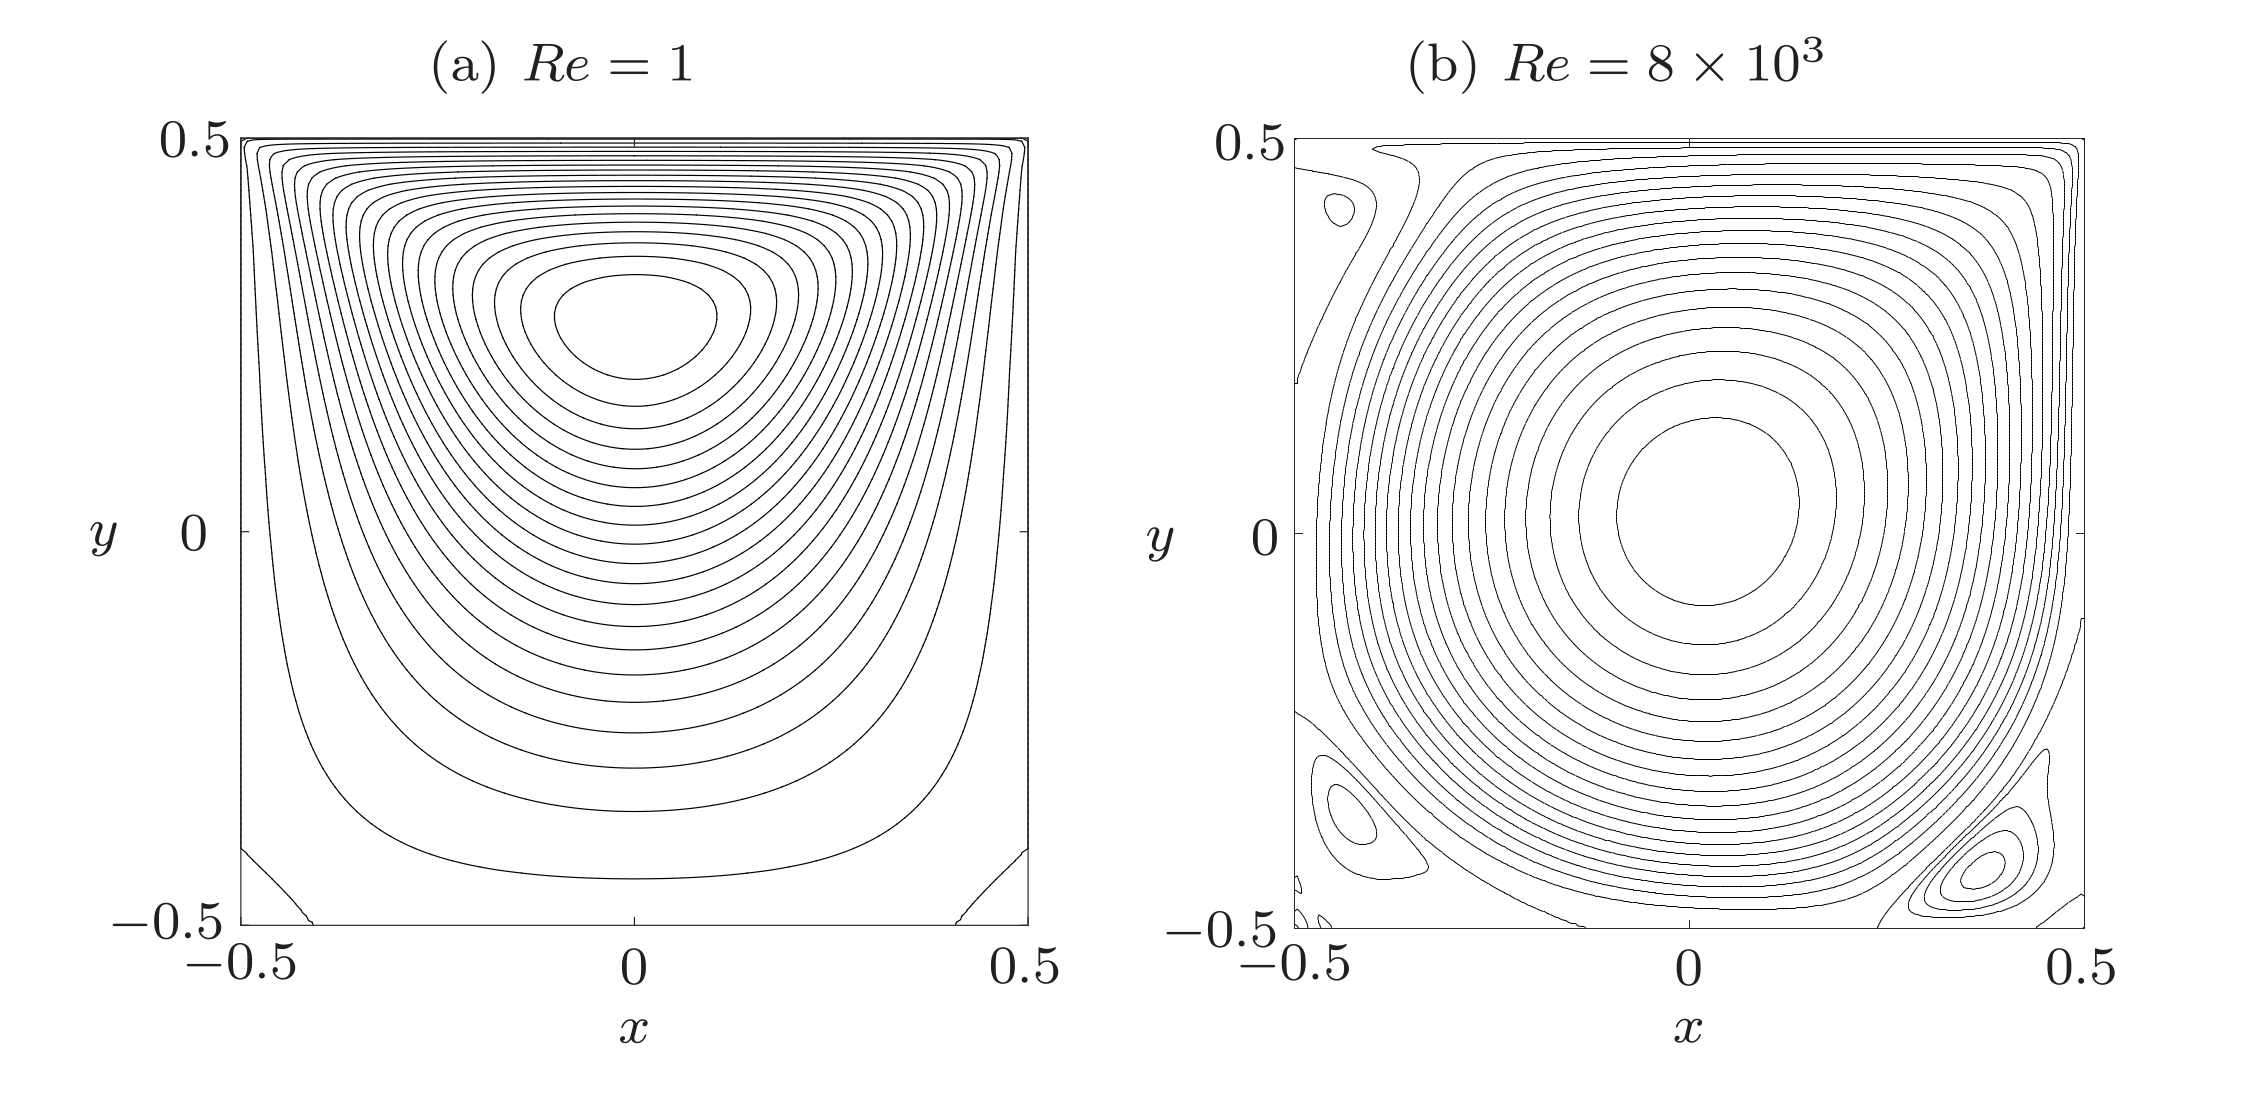
\includegraphics[width=0.7\textwidth]{figs/fig_kuhlmann2019}
\end{center}
\caption{Isolines of the streamfunction of the lid-driven cavity at Reynolds
  numbers 1 (a) and 8000 (b), figures adapted from \cite{kuhlmann2019}}
\label{fig:Re_cav_simple}
\end{figure}

The flow phenomena in the upper corners result from the discontinuous boundary
conditions of the mathematical problem. These are caused by the horizontal
component being set to a velocity $U$ at the upper corners, but on the
contrary, the vertical walls are not moving. What follows is that the pressure
and the vorticity diverge at these corners. This phenomenon is a special case
of Taylor's scrapper problem, and there exists a closed-form solution in terms
of series expansions \citep{kuhlmann2019}. The other effect worth mentioning is
the formation of two eddies at the lower corners of the cavity. These vortices
rotate in an anti-clockwise way, separated from the central vortex. They are
called Moffat eddies, and similarity solutions have been found for them
\citep{moffatt1964}.

Apart from these studies, calculating the solutions of the cavity while varying
the Reynolds number has been done extensively. The single lid-driven cavity
becomes unstable at a Hopf bifurcation (see section \ref{sec:bif}) somewhere in
the range of the Reynolds number [7500, 8100] \citep{kuhlmann2019} conducted by
different studies. No conclusive results could be drawn due to the significant
uncertainty. The numerical deviations come mainly from the large Reynolds
number at which the bifurcations appear and the different discretization used
to obtain the results. Another main issue, as mentioned before, is the corner
singularities caused by discontinuous boundary conditions.

Until now, we have restricted our attention only to the simple 2D single
lid-driven case. However, there is a whole spectrum of different variants.
First, the analysis can be performed for different aspect ratios (height-width
of the box) and evaluate the effect on the flow pattern. Other shapes apart
from a rectangular cavity can be considered as well. With more computing
resources being available, the 3D variant has also been studied, giving rise to
other types of singularities and flow patterns \citep{lopez2017}. Lastly, the
problem can be combined with heat convection by keeping facing sides at
different temperatures \citep{koseff1985}. \\

In this work, we want to consider another type of flow variant by adapting the
boundary conditions. \cite{kuhlmann1997} investigated numerically and
experimentally a two-sided flow problem where two opposing lids move in
opposite directions. It has been found that the primary symmetric flow pattern
is only stable for low Reynolds numbers, and the flow becomes unstable at a
large Reynolds number because of a three-dimensional mode. \citep{wahba2009}
did further numerical experiments and proposed an extension, the four-sided
version (figure \ref{fig:cav_4s}), where all four walls are moving at different
speeds (top-bottom and right-left lids moving rightwards-leftwards and
upwards-downwards, respectively). This problem exhibits bifurcations from a
very low Reynolds number onward. Figure \ref{fig:bc_types} shows the different
types of boundary conditions.

\begin{figure}[ht]
\centering
\begin{subfigure}[b]{0.3\textwidth}
  \centering
  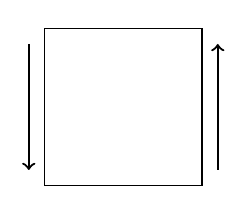
\begin{tikzpicture}[scale=2]
    \draw (0,0) rectangle (1,1);
    \draw[thick, ->] (-0.1,0.9) -- (-0.1,0.1);
    \draw[thick, ->] (1.1,0.1) -- (1.1,0.9);
  \end{tikzpicture}
  \caption{Two-sided lid-driven cavity \\ \hspace{\textwidth}}
  \label{subfig:bc_2s}
\end{subfigure}
\begin{subfigure}[b]{0.3\textwidth}
  \centering
  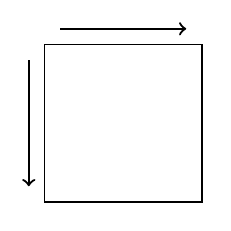
\begin{tikzpicture}[scale=2]
    \draw (0,0) rectangle (1,1);
    \draw[thick, ->] (-0.1,0.9) -- (-0.1,0.1);
    \draw[thick, ->] (0.1,1.1) -- (0.9,1.1);
  \end{tikzpicture}
  \caption{Two-sided lid-driven cavity (non-facing)}
  \label{subfig:bc_2s_nf}
\end{subfigure}
\begin{subfigure}[b]{0.3\textwidth}
  \centering
  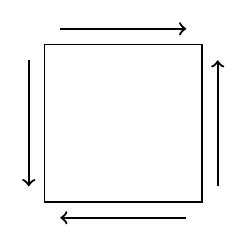
\begin{tikzpicture}[scale=2]
    \draw (0,0) rectangle (1,1);
    \draw[thick, ->] (0.1,1.1) -- (0.9,1.1);
    \draw[thick, ->] (1.1,0.1) -- (1.1,0.9);
    \draw[thick, ->] (0.9,-0.1) -- (0.1,-0.1);
    \draw[thick, ->] (-0.1,0.9) -- (-0.1,0.1);
  \end{tikzpicture}
  \caption{Four-sided lid-driven cavity \\ \hspace{\textwidth}}
  \label{subfig:bc_4s}
\end{subfigure}

\caption{Variations of the boundary conditions for the cavity flow,
 with  the moving lids set to equal speeds $U$}
\label{fig:bc_types}
\end{figure}

\subsection{Regularization} \label{sec:regul}

The corner singularities pose a well-known problem, and applying analytic
insights of the 2D case can give rise to more precise calculations.
\cite{botella1998} used spectral methods (see section \ref{sec:spectral}) in
combination with the substraction of the leading terms of the singularities. In
this way, the numerically solved problem does not involve singularities, and
the global discretization of spectral methods can safely be applied and gives
highly accurate results. 

Another successful strategy is to adapt the boundary condition to study a more
well-posed problem. Regularized versions of the boundary conditions are used to
replace discontinuous velocity profiles. The velocity is set to zero at the
corners and increases to the desired value at the boundary. To construct such
regularization functions, polynomials \citep{shen1991} and trigonometric
functions have been tested in the literature. \cite{shen1991} used 4-th order
polynomials, which seem to be too low of an order and give different results
compared to the original problem. A more recent regularization function
involves exponentials \citep{lopez2017} which was applied to a 3D problem and
seems to work well to represent the constant velocity at the lid and still be
smooth function at all the corners.

Resembling the original problem through regularized functions can recover the
exponential convergence of spectral discretizations. The resolution of the
bifurcation points can thus be calculated more reliably.  

\subsection{The four-sided lid-driven Cavity Flow} \label{sec:4sc}

\begin{figure}[ht]
\centering
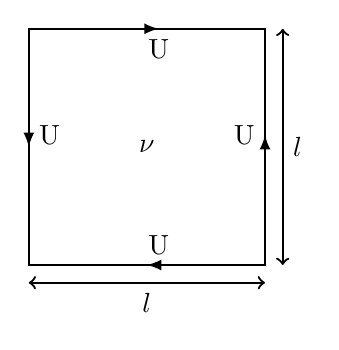
\begin{tikzpicture}[scale=1.5]
  \draw[thick] (0,0) rectangle (2,2);
  \draw[thick] (0,0) rectangle (2,2);

  \node at (1,1) {$\nu$};

  \draw[-latex, thick] (2,0) -- node[pos=0.9, above] {U} (1,0);
  \draw[-latex, thick] (0,2) -- node[pos=0.9, right] {U} (0,1);
  \draw[-latex, thick] (2,0) -- node[pos=1, left] {U} (2,1.1);
  \draw[-latex, thick] (0,2) -- node[pos=1, below] {U} (1.1,2);

  \draw[<->, thick] (0,-0.15) -- node[pos=0.5, below] {$l$} (2,-0.15);
  \draw[<->, thick] (2.15,0) -- node[pos=0.5, right] {$l$} (2.15,2);
\end{tikzpicture}
\caption{The four-sided cavity ($l \times l$) with tangential velocities $U$ and
  kinematik viscosity $\nu$ }
\label{fig:cav_4s}
\end{figure}

In the paper of \cite{wahba2009}, a multiplicity of states in the four-sided
lid-driven cavity flows have been discovered. The numerical simulations have
been carried out on a finite-difference grid with the line successive
over-relaxation method (LSOR) to compute the results. The study reveals the
presence of multiple steady solutions and exhibits interesting flow
bifurcations at low to moderate Reynolds numbers. The flow is symmetric at
first, and then two stable asymmetric solutions appear, whereas the symmetric
solution becomes unstable. See figure \ref{fig:4fsc_states} for the
visualization of these states.

\begin{figure}[ht]
  \centering
  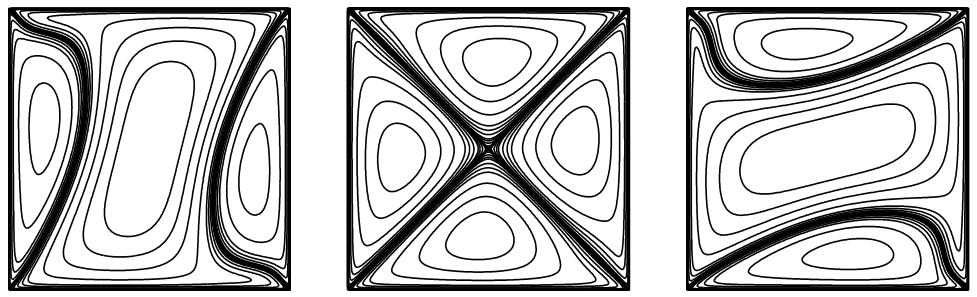
\includegraphics[width=0.455\textwidth]{figs/fig_wahba2009}
  \caption{Symmetric and asymmetric solutions at $Re=300$, computed by
    \cite{wahba2009}}
  \label{fig:4fsc_states}
\end{figure}

Later, \cite{perumal2011} employed a Lattice Boltzmann Method (LBM), recovering
multiple solutions obtained by the former finite-difference based code.
Furthermore, other aspect ratios for cavities have been considered, which
exhibit the multiplicity of solutions as well. 

\begin{figure}[ht]
  \centering
  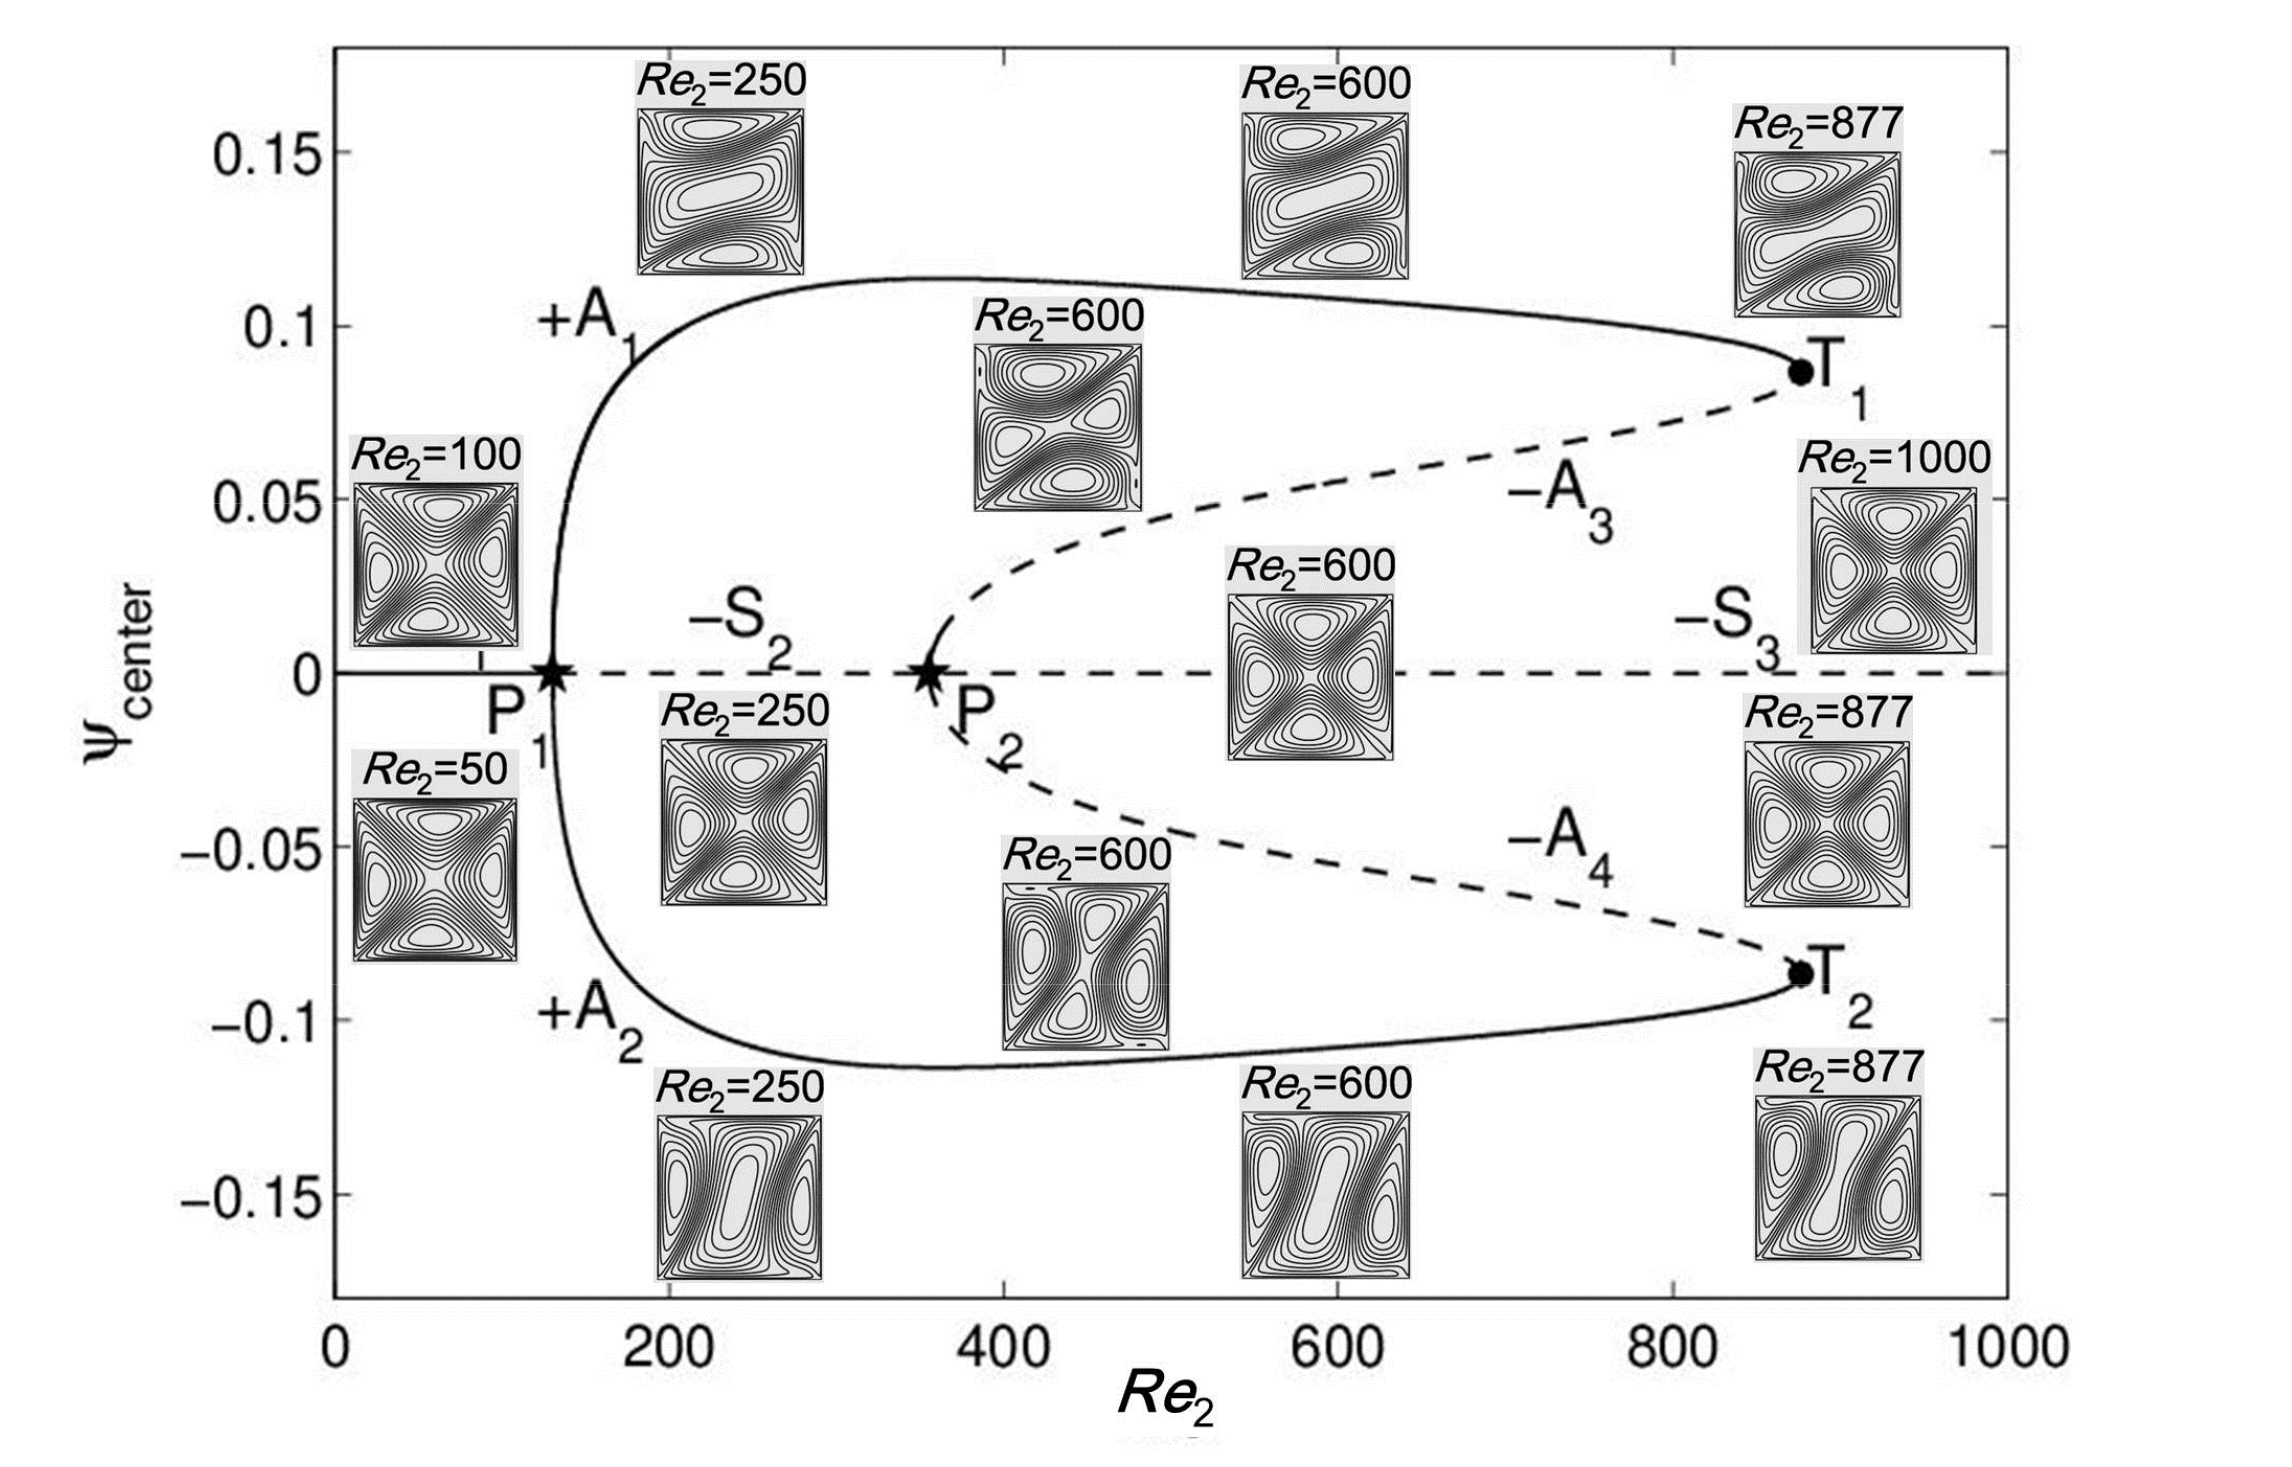
\includegraphics[width=0.8\textwidth]{figs/fig2_chen2013.png}
  \caption{Bifurcation diagram obtained by \cite{chen2013} for the
    non-regularized four-sided cavity flow, Reynolds numbers are 
    double the results obtained in this study} 
  \label{fig:bif_diag_chen}
\end{figure}

\cite{cadou2012} developed numerical tools for the stability analysis in two-
and four-sided lid-driven cavity flows. They recognized a secondary bifurcation
point at a higher Reynolds number where the symmetric solution is stable again.
Equally, the two-sided cavity flow has been changed to have non-facing moving
lids (figure \ref{subfig:bc_2s_nf}). In this asymmetric problem a Hopf
bifurcation has been discovered. On the other hand, in the four-sided version,
no such bifurcation has been reported in the literature.

A full bifurcation diagram (figure \ref{fig:bif_diag_chen}) was presented by
\cite{chen2013}, where the streamfunction value at the center of the cavity is
plotted against an increasing Reynolds number. Through a continuation
algorithm, the asymmetric solution branches could be followed (see section
\ref{sec:bif}) and are visualized in the diagram. The solid curves represent
stable solutions, whereas the dashed curves correspond to unstable ones. One
notices that the effect of changing the Reynolds in the four-sided reveals two
pitchfork bifurcations and saddle node (fold) points for the asymmetric
solutions. Apart from the LBM technique in \citet{chen2013}, the domain has
been discretized with finite differences, and as pointed out in the section
\ref{sec:regul}, the goal here is to look at a regularized problem with the aim
of using spectral discretization.

The governing equations will now be introduced formally and the more well-posed
boundary conditions will be defined to achieve higher accuracy and an
exponential convergence rate.
